% Chapter 3. Update when a method, setting or threshold changes (record the old value too).
\chapter{Methods}
\label{ch:methods}

This chapter describes the workflow in the order in which it was built. Each stage was tested
before the next one started, and later stages reuse the code of earlier ones.
\Cref{tab:stages} lists the stages, and \cref{fig:pipeline} shows how the parts fit together in
the final evolutionary loop.

\begin{table}[ht]
  \centering
  \caption{Stages of the work. Each stage has its own folder and README in the project
           repository.}
  \label{tab:stages}
  \small
  \begin{tabularx}{\textwidth}{@{}lLl@{}}
    \toprule
    Stage & What it adds & Section \\
    \midrule
    0  & LangGraph agent with an LLM, a software check, five validation steps and saving & \ref{sec:agent} \\
    1  & Conversion between hexagon lists and molecules; the 91{,}174-structure dataset in hexagon form & \ref{sec:hex} \\
    2  & Machine-learned predictor of the xTB gap with uncertainty & \ref{sec:predictor} \\
    2d & LLM designs GQDs as hexagon lists; closed-shell rule and fix feedback & \ref{sec:hex}, \ref{sec:e1} \\
    3a & \ce{NO2} sensing score from GFN2-xTB; DFT check on small models & \ref{sec:score}, \ref{sec:dft-methods} \\
    3  & Evolutionary loop with LLM or random mutation; pilot run & \ref{sec:loop} \\
    4  & Comparison with three runs per mutator; GPU DFT benchmark & \ref{sec:e4}, \ref{sec:e5} \\
    \bottomrule
  \end{tabularx}
\end{table}

\begin{figure}[ht]
  \centering
  \begin{tikzpicture}[node distance=7mm and 9mm,
      box/.style={draw, rounded corners=2pt, align=center, font=\small, minimum height=11mm,
                  text width=31mm, fill=#1}, box/.default=white,
      arr/.style={-{Stealth[length=2.2mm]}, thick}]
    \node[box=blue!8] (mut) {Mutator\\(LLM or random)};
    \node[box, right=of mut] (edit) {Child = parent\\+ 1 to 3 hexagon edits};
    \node[box=green!8, right=of edit] (val) {Code builds and\\validates (and repairs)};
    \node[box=green!8, below=of val] (pre) {Gap pre-filter\\(ML predictor)};
    \node[box=orange!12, left=of pre] (xtb) {xTB sensing score\\(\ce{NO2} and CO)};
    \node[box=blue!8, left=of xtb] (sel) {Selection: best 8,\\at most 3 per family};
    \node[box=gray!10, below=of xtb] (dft) {DFT check of\\selected GQDs (GPU)};
    \draw[arr] (mut) -- (edit);
    \draw[arr] (edit) -- (val);
    \draw[arr] (val) -- (pre);
    \draw[arr] (pre) -- (xtb);
    \draw[arr] (xtb) -- (sel);
    \draw[arr] (sel) -- (mut);
    \draw[arr, dashed] (val.north) -- ++(0,6mm) -| node[pos=0.25, above, font=\scriptsize]
      {rejected: reason and fix edits} (mut.north);
    \draw[arr, dashed] (xtb) -- (dft);
  \end{tikzpicture}
  \caption{One generation of the evolutionary loop. The mutator proposes children as edits of
           the current best GQDs. Code turns each child into a molecule, checks it, and sends
           rejections back with the reason. A free ML prediction of the gap removes children
           outside a useful range, and GFN2-xTB scores the rest. The best GQDs scored so far
           become the next parents. Every proposal is logged, and selected GQDs are checked
           with DFT outside the loop.}
  \label{fig:pipeline}
\end{figure}

% ==========================================================================================
\section{The agent and its validation chain}
\label{sec:agent}

The project started as an agent built with LangGraph \cite{langgraph}, a library that describes an
LLM application as a graph of nodes that share a state. Before the agent, two small LangGraph
examples and a three-node graph that only read candidates from a table were written to learn the
library. The agent itself (\code{studio/agent.py}) is shown in \cref{fig:agent}.

The first node checks that the required software is present: the Python packages RDKit
\cite{rdkit}, NumPy, SciPy, PySCF \cite{sun2018pyscf} and geomeTRIC, and the \code{xtb} program. If
something is missing, the agent stops and says what is missing. Otherwise control passes to the
assistant node, where the LLM reads the conversation and either answers or calls a tool. The LLM is
GPT-5.4, accessed through an Azure OpenAI deployment (API version 2024-02-01) with LangChain
\cite{langchain}. Only one tool call is allowed per turn, because the validation nodes check one
structure at a time.

The agent has two tools. The first, \code{generate\_gqd}, returns a random SMILES string from a
pilot table of the existing dataset. It stood in for a structure generator while the graph was
being built. The second, \code{build\_gqd\_from\_hexagons}, lets the LLM design a GQD itself by
writing hexagon positions (\cref{sec:hex}).

Every structure that a tool returns passes through five checks in a fixed order:
\begin{enumerate}
  \item \emph{Molecular graph.} RDKit must parse and sanitise the SMILES, and the molecule must be
        one connected piece. Errors from the hexagon tool, such as an open-shell design, are
        reported at this step.
  \item \emph{Uniqueness.} The InChIKey must not already be among the saved structures.
  \item \emph{Ring count.} The molecule must have 20 to 40 six-membered rings.
  \item \emph{Hybridisation.} At least 95\% of the heavy atoms must be \(sp^2\).
  \item \emph{Synthetic accessibility.} The SA score \cite{ertl2009sascore} must be 8.0 or lower.
\end{enumerate}
These thresholds are the ones used to generate the original dataset. A structure that passes all
five is saved to a table together with a \code{.mol} file. A structure that fails goes back to the
LLM with the name of the failed step and the reason. The system prompt asks the LLM to fix its own
rejected designs and to give up after three rejections for the same request.

\begin{figure}[ht]
  \centering
  \begin{tikzpicture}[font=\small, node distance=8mm,
      st/.style={draw, rounded corners=2pt, align=center, minimum height=7mm, text width=#1,
                 inner sep=3pt},
      arr/.style={-{Stealth[length=2mm]}, thick},
      lab/.style={font=\scriptsize, align=center}]
    \node[draw, circle, inner sep=1.5pt, font=\scriptsize] (start) {start};
    \node[st=22mm, fill=gray!10, right=6mm of start] (sw) {software\\check};
    \node[st=22mm, fill=blue!8, right=of sw] (llm) {assistant\\(LLM)};
    \node[st=42mm, fill=orange!12, right=14mm of llm] (tools)
      {tool call\\{\scriptsize\code{build\_gqd\_from\_hexagons}}};
    \node[st=42mm, fill=green!8, below=5mm of tools] (c1) {1. molecular graph (RDKit)};
    \node[st=42mm, fill=green!8, below=3mm of c1] (c2) {2. new (InChIKey)};
    \node[st=42mm, fill=green!8, below=3mm of c2] (c3) {3. 20 to 40 hexagons};
    \node[st=42mm, fill=green!8, below=3mm of c3] (c4) {4. \(sp^2\) fraction \(\geq 0.95\)};
    \node[st=42mm, fill=green!8, below=3mm of c4] (c5) {5. SA score \(\leq 8.0\)};
    \node[st=42mm, fill=gray!10, below=6mm of c5] (save) {save (table and \code{.mol} file)};
    \begin{scope}[on background layer]
      \node[draw, dashed, rounded corners, fit=(c1)(c5), inner sep=2mm] (checks) {};
    \end{scope}
    \node[draw, circle, inner sep=1.5pt, font=\scriptsize, above=7mm of llm] (end) {end};
    \draw[arr] (start) -- (sw);
    \draw[arr] (sw) -- (llm);
    \draw[arr] (llm) -- node[lab, above] {tool call} (tools);
    \draw[arr] (tools) -- (c1);
    \draw[arr] (c1) -- (c2);
    \draw[arr] (c2) -- (c3);
    \draw[arr] (c3) -- (c4);
    \draw[arr] (c4) -- (c5);
    \draw[arr] (c5) -- (save);
    \draw[arr] (llm) -- node[lab, right] {answer} (end);
    \draw[arr] (sw.north) |- node[lab, pos=0.3, left] {missing\\software} (end.west);
    \draw[arr, dashed] (checks.west) -| node[lab, pos=0.78, right] {rejected:\\step and\\reason}
      ([xshift=4mm]llm.south);
    \draw[arr] (save.west) -| node[lab, pos=0.2, above] {accepted} ([xshift=-4mm]llm.south);
  \end{tikzpicture}
  \caption{The agent as a LangGraph state graph. The LLM proposes, and code decides: every
           structure passes the five checks in order, and a failure returns the step and the
           reason to the LLM.}
  \label{fig:agent}
\end{figure}

The agent established the rule that the rest of the work follows: the LLM may propose anything,
but only code decides whether a structure is accepted.

% ==========================================================================================
\section{Hexagon representation of GQDs}
\label{sec:hex}

\subsection{Coordinates}

A GQD is a set of fused hexagons on a honeycomb lattice, so it can be written as the list of
hexagons it occupies (\cref{fig:hexgrid}a). We use axial coordinates \((q,r)\). The six neighbours
of hexagon \((q,r)\) are \((q\pm1,r)\), \((q,r\pm1)\), \((q+1,r-1)\) and \((q-1,r+1)\). Benzene is
\([(0,0)]\), naphthalene is \([(0,0),(1,0)]\), and coronene is \((0,0)\) with its six neighbours.
In this form the number of rings is the length of the list, two hexagons are fused when they are
neighbours, and an edit to the shape is the addition or removal of one entry. The coordinate
convention and the rules for corners are the same as in the generator that produced the original
dataset.

\begin{figure}[ht]
  \centering
  \begin{subfigure}[b]{0.34\textwidth}
    \centering
    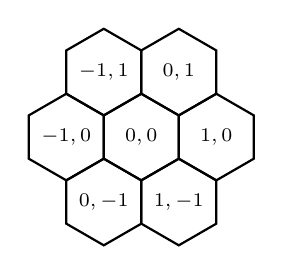
\begin{tikzpicture}[x=5.5mm, y=5.5mm]
      \foreach \qq/\rr in {0/0, 1/0, -1/0, 0/1, 0/-1, 1/-1, -1/1} {
        \begin{scope}[shift={({sqrt(3)*(\qq+0.5*(\rr))}, {1.5*(\rr)})}]
          \draw[thick] (90:1) -- (30:1) -- (-30:1) -- (-90:1) -- (-150:1) -- (150:1) -- cycle;
          \node[font=\scriptsize] at (0,0) {\(\qq,\rr\)};
        \end{scope}
      }
    \end{tikzpicture}
    \caption{Coronene, with \((q,r)\) of each hexagon.}
  \end{subfigure}\hfill
  \begin{subfigure}[b]{0.30\textwidth}
    \centering
    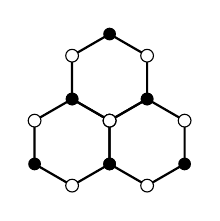
\begin{tikzpicture}[x=5.5mm, y=5.5mm]
      \foreach \qq/\rr in {0/0, 1/0, 0/1} {
        \begin{scope}[shift={({sqrt(3)*(\qq+0.5*(\rr))}, {1.5*(\rr)})}]
          \draw[thick] (90:1) -- (30:1) -- (-30:1) -- (-90:1) -- (-150:1) -- (150:1) -- cycle;
        \end{scope}
      }
      \foreach \qq/\rr in {0/0, 1/0, 0/1} {
        \begin{scope}[shift={({sqrt(3)*(\qq+0.5*(\rr))}, {1.5*(\rr)})}]
          \foreach \a in {90, 210, 330} \fill (\a:1) circle (2.3pt);
          \foreach \a in {30, 150, 270} \filldraw[fill=white, draw=black] (\a:1) circle (2.3pt);
        \end{scope}
      }
    \end{tikzpicture}
    \caption{Phenalenyl: 7 white and 6 black atoms. Open-shell.}
  \end{subfigure}\hfill
  \begin{subfigure}[b]{0.30\textwidth}
    \centering
    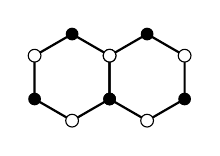
\begin{tikzpicture}[x=5.5mm, y=5.5mm]
      \foreach \qq/\rr in {0/0, 1/0} {
        \begin{scope}[shift={({sqrt(3)*(\qq+0.5*(\rr))}, {1.5*(\rr)})}]
          \draw[thick] (90:1) -- (30:1) -- (-30:1) -- (-90:1) -- (-150:1) -- (150:1) -- cycle;
        \end{scope}
      }
      \foreach \qq/\rr in {0/0, 1/0} {
        \begin{scope}[shift={({sqrt(3)*(\qq+0.5*(\rr))}, {1.5*(\rr)})}]
          \foreach \a in {90, 210, 330} \fill (\a:1) circle (2.3pt);
          \foreach \a in {30, 150, 270} \filldraw[fill=white, draw=black] (\a:1) circle (2.3pt);
        \end{scope}
      }
    \end{tikzpicture}
    \caption{Naphthalene: 5 white and 5 black atoms. Closed-shell.}
  \end{subfigure}
  \caption{The hexagon representation. (a) Axial coordinates. (b, c) The carbon atoms split into
           two sublattices (black and white), and every bond joins a black atom to a white one. A
           Kekul\'e structure needs equal numbers of the two, so the three-ring triangle in (b)
           must be a radical, while (c) is closed-shell.}
  \label{fig:hexgrid}
\end{figure}

\subsection{From hexagons to a molecule}

\Cref{alg:hex2mol} converts a hexagon list into an RDKit molecule. Each hexagon has six corners,
and a corner is named by the three grid positions that meet at it, so a corner shared by fused
hexagons becomes a single carbon atom. Each hexagon edge becomes a carbon-carbon bond, and each
carbon with only two carbon neighbours receives one hydrogen.

The double bonds are chosen by the code rather than by RDKit. A Kekul\'e structure is a perfect
matching of the carbon graph, and because the graph is bipartite, the augmenting-path method of
Kuhn \cite{kuhn1955hungarian} finds one or proves that none exists. We do this ourselves because
RDKit's kekulisation failed for some large GQDs depending on the order of the atoms: the same
structure passed or failed when its hexagons were listed in a different order. If no perfect
matching exists, the design is open-shell and is rejected. After sanitisation, the SMILES string
is written and read back. RDKit cannot re-read the SMILES of some valid closed-shell shapes, and
because every later step reads SMILES with RDKit, these shapes are rejected too
(\cref{sec:res-hex}).

The reverse function, \code{mol\_to\_hex}, places the first six-membered ring at \((0,0)\) and
walks across shared bonds: a ring that shares edge \(k\) of a placed hexagon must sit at the
neighbouring grid position for that edge. It returns the hexagon list or raises an error if the
rings do not fit on a flat honeycomb grid. A hexagon-sized hole has the same atoms and bonds as a
filled hexagon, so \code{mol\_to\_hex} returns such a structure with the hole filled.

\begin{algorithm}[ht]
  \caption{Hexagon list to molecule (\code{hex\_to\_mol})}
  \label{alg:hex2mol}
  \begin{algorithmic}[1]
    \Require list \(H\) of hexagon positions \((q,r)\); size range \([20,40]\)
    \State check that \(H\) has integer pairs, no duplicates and one connected piece
           \Comment{else reject}
    \For{each hexagon \(h \in H\) and each of its six corners}
      \State key \(\gets\) the three grid positions that meet at the corner
      \State create one carbon per distinct key; add a bond for each hexagon edge
    \EndFor
    \State \(M \gets\) perfect matching of the carbon graph (augmenting paths)
    \If{no perfect matching exists}
      \State \(N_A, N_B \gets\) sublattice counts; \(F \gets\) fix edits (\cref{alg:fixes})
      \State \textbf{reject} with ``open-shell, \(N_A\) vs \(N_B\)'' and the edits in \(F\)
    \EndIf
    \State make the bonds in \(M\) double and the rest single; add H to two-coordinate carbons
    \State sanitise with RDKit; write the SMILES and read it back \Comment{else reject}
    \State \Return the molecule
  \end{algorithmic}
\end{algorithm}

\subsection{Explaining an open-shell design}

An LLM cannot see the sublattice balance in a list of coordinates. When a design is open-shell, a
message such as ``no Kekul\'e form'' does not tell it what to change. The rejection message
therefore states the imbalance (for example ``33 vs 28, 5 unpaired atoms'') and lists concrete
edits that fix it (\cref{alg:fixes}). A corner belongs to sublattice A when the sum of \(q+r\) over
the three grid positions that meet there is 1 modulo 3, which makes the counts cheap to compute.
The code first tries every single edit, either adding a hexagon at an empty neighbouring position
or removing a hexagon whose removal keeps the shape connected, and keeps up to six edits that give
a closed-shell structure of allowed size. If no single edit works, a beam search (width 30) over
edit sequences of up to eight steps, ranked by the remaining imbalance \(|N_A-N_B|\), returns the
shortest sequence it finds. Every suggestion is checked with the exact matching test, and the
search takes about 0.1 to 0.5~s. The LLM still decides which edit to apply.

\begin{algorithm}[ht]
  \caption{Fix edits for an open-shell design (\code{open\_shell\_fixes})}
  \label{alg:fixes}
  \begin{algorithmic}[1]
    \Require open-shell hexagon set \(H\); size range \([20,40]\)
    \State \(E(H) \gets\) all single edits: add an empty neighbour, or remove a hexagon if the rest
           stays connected, within the size range
    \State \(F \gets \{e \in E(H) : H \oplus e \text{ has a Kekul\'e structure}\}\)
    \If{\(F \neq \emptyset\)}
      \State \Return up to six edits from \(F\)
    \EndIf
    \State frontier \(\gets \{(\,(),\,H)\}\)
    \For{depth \(= 1\) to 8}
      \For{each \((\text{path}, S)\) in frontier and each \(e \in E(S)\) not seen before}
        \If{\(S \oplus e\) has a Kekul\'e structure}
          \State \Return path \(+\,e\)
        \EndIf
      \EndFor
      \State frontier \(\gets\) the 30 new shapes with the smallest \(|N_A - N_B|\)
    \EndFor
    \State \Return no fix found
  \end{algorithmic}
\end{algorithm}

\subsection{The closed-shell rule in the prompt}
\label{sec:rule-prompt}

The second aid is a paragraph in the system prompt (\cref{app:prompts}). It explains that the
carbon atoms form two alternating sets that must be equal in number, names the shapes that usually
break this rule (triangles, L-shaped corners and long zigzag edges), and gives a simple way to
satisfy it: make the shape point-symmetric, so that for every \([q,r]\) the list also contains
\([a-q,b-r]\) for a fixed centre \((a/2,b/2)\). The centre of such an inversion is either a hexagon
centre or the midpoint of a shared bond, and in both cases the inversion maps every atom of one
sublattice onto an atom of the other, so the two counts are equal. Equal counts do not guarantee a
Kekul\'e structure, but in practice they remove most failures (\cref{sec:res-e1}).

\subsection{The dataset in hexagon form}

The existing dataset contains 91{,}174 GQDs with 20 to 40 hexagons, generated earlier in the
project by growing random hexagon clusters, given as SMILES. Each structure was converted to a
hexagon list with \code{mol\_to\_hex}, converted back with \code{hex\_to\_mol}, and kept only if
the canonical SMILES matched. Where available, xTB values of the HOMO, LUMO and gap were attached;
14{,}674 structures have them (4{,}600 from a first xTB batch and 10{,}074 from a second).

% ==========================================================================================
\section{Fast gap predictor}
\label{sec:predictor}

An xTB calculation takes minutes, while a prediction from a trained model takes milliseconds. The
predictor estimates the GFN2-xTB HOMO-LUMO gap of a GQD from its hexagon list or SMILES, together
with an uncertainty \(\sigma\). In the loop it is a free filter that removes children whose
gap is outside a useful range.

\paragraph{Data.} The 14{,}674 xTB-labelled GQDs were split 80/10/10 into training, validation and
test sets, stratified by gap. The 1{,}468 test structures were used only for the final report.

\paragraph{Baseline and features.} The H\"uckel gap, computed from the eigenvalues of the carbon
adjacency matrix, correlates with the xTB gap at \(r = 0.984\). A linear fit,
\(\Delta_{\mathrm{xTB}} \approx 2.5477\,\Delta_{\mathrm{H}} + 0.0527\)~eV with \(\Delta_{\mathrm{H}}\)
in units of \(|\beta|\), is the baseline, and the learned models predict only the residual. They
use 49 physics-based features: the H\"uckel spectrum near the gap (orbital energies, neighbouring
gaps, near-zero levels, orbital localisation and edge weight of the frontier orbitals), the
number of Kekul\'e structures and the Clar number, edge hydrogen types, perimeter features (bays,
coves, fjords), holes, and size and shape descriptors. A 2{,}048-bit Morgan fingerprint alone
reached only \(R^2 = 0.36\), so the physics features carry most of the signal.

\paragraph{Models.} LightGBM and XGBoost \cite{ke2017lightgbm,chen2016xgboost} were tuned with
Optuna \cite{akiba2019optuna} (100 trials each). A graph neural network in the style of GIN
\cite{xu2019gin} uses one node per carbon, with node features for edge position, ring membership,
hole contact and frontier-orbital coefficients, and receives the 49 features as global inputs.
Each model type was trained in five-fold cross-validation, and the fold models are averaged at
prediction time. Out-of-fold predictions set the ensemble weights (0.85 GNN and 0.15 XGBoost).

\paragraph{Uncertainty.} A LightGBM error model predicts the expected absolute error from the
features and from the disagreement between the models. It is scaled by 1.54 so that
\(\pm1.96\sigma\) covers 95\% of the out-of-fold errors. Inputs with fewer than 20 or more than
40 hexagons are refused, because the model is not valid there.

% ==========================================================================================
\section{\NOtwo{} sensing score}
\label{sec:score}

\subsection{Requirements}

A good \ce{NO2} sensing material has to meet three requirements. It must \emph{respond}: \ce{NO2}
should take electrons from the GQD, which changes the conductance of the layer, and more charge
means a larger signal. It must \emph{recover}: \ce{NO2} should not bind so strongly that it never
leaves. And it must be \emph{selective}: \ce{NO2} should bind more strongly than the other gases in
air, here water, ammonia and carbon monoxide. The function \code{evaluate\_gqd}
(\cref{alg:evaluate}) turns these requirements into numbers that GFN2-xTB can compute for any
hexagon list.

\subsection{Geometry and calculations}

The starting geometry of the GQD is built from the hexagon grid with \ce{C-C} bonds of 1.42~\AA{} and
\ce{C-H} bonds of 1.09~\AA{}. A small random out-of-plane displacement is added to every atom,
drawn from a normal distribution with a standard deviation of 0.05~\AA. The random generator is
seeded from the hexagon list, so the same GQD always starts from the same geometry. Most
GQDs in the dataset have crowded edges (coves or fjords) and are twisted at their minimum, and a
perfectly flat start gives the optimiser no force out of the plane; \cref{sec:res-flat} shows what
went wrong without the displacement. The GQD is then optimised with GFN2-xTB.

Two adsorption sites are probed: the hexagon closest to the centre of the GQD, and the most exposed
edge hexagon, defined as the hexagon with the fewest neighbours (ties broken by distance from the
centre). Each gas is placed above the centre of the site hexagon with its lowest atom 3.1~\AA{}
above the GQD plane. \ce{NO2} is placed in two orientations, with nitrogen down and with oxygen
down. \ce{H2O}, \ce{NH3}, CO and \ce{O2} use one orientation each. This gives 12 complexes, which
are optimised with GFN2-xTB in parallel. \ce{NO2} is a doublet and \ce{O2} a triplet, so these
complexes are computed with one and two unpaired electrons.

\subsection{Descriptors}

For each complex, the adsorption energy is
\begin{equation}
  \Eads = E(\text{GQD}+\text{gas}) - E(\text{GQD}) - E(\text{gas}),
  \label{eq:eads}
\end{equation}
where all three energies are from optimised structures. For each gas, the site and orientation
with the most negative \(\Eads\) are kept. From the \ce{NO2} complex we record the charge on the
\ce{NO2} atoms (the sum of the xTB atomic partial charges) and the shortest distance between the
gas and the GQD. A contact shorter than 1.9~\AA{} means that a covalent bond has formed, and the
\ce{NO2} is called chemisorbed. The recovery time is estimated as
\begin{equation}
  \tau = \nu^{-1}\exp\!\left(-\Eads/k_BT\right), \qquad \nu = 10^{12}~\text{s}^{-1},\; T = 298.15~\text{K}.
  \label{eq:tau}
\end{equation}

\subsection{Score}

The score multiplies a response term by two factors between 0 and 1:
\begin{align}
  S &= q_{\ce{NO2}} \times R \times \Sigma, \label{eq:score}\\
  R &= \operatorname{clip}\!\left(\frac{E_{\ce{NO2}} - E_{\mathrm{hard}}}{E_{\mathrm{soft}} - E_{\mathrm{hard}}},\,0,\,1\right),
      \qquad E_{\mathrm{soft}} = -0.6~\text{eV},\; E_{\mathrm{hard}} = -1.0~\text{eV}, \label{eq:rev}\\
  \Sigma &= \operatorname{clip}\!\left(\frac{\min_{g} E_g - E_{\ce{NO2}}}{0.10~\text{eV}},\,0,\,1\right),
      \qquad g \in \{\ce{H2O}, \ce{NH3}, \ce{CO}\}. \label{eq:sel}
\end{align}
Here \(q_{\ce{NO2}}\) is the number of electrons that move to \ce{NO2} (in units of \(e\)), and
\(E_{\ce{NO2}}\) and \(E_g\) are the strongest adsorption energies of \ce{NO2} and of each
interfering gas. The reversibility factor \(R\) is 1 when \ce{NO2} binds no more strongly than
\(-0.6\)~eV and falls linearly to 0 at \(-1.0\)~eV. By \cref{eq:tau}, recovery takes about 0.3~ms
at 0.5~eV, 7~s at 0.76~eV, 27~min at 0.9~eV and 22~h at 1.0~eV. The window is set somewhat lower
than a pure recovery argument would suggest because GFN2-xTB overbinds chemisorbed \ce{NO2} by 0.1
to 0.55~eV compared with DFT (\cref{sec:res-dft-small}). The selectivity factor \(\Sigma\) is 1
when \ce{NO2} binds at least 0.10~eV more strongly than the strongest interfering gas. \ce{O2} is
computed but not used in the score, because xTB describes it wrongly (\cref{sec:res-dft-small}).
The score has units of \(e\), and higher is better.

\begin{algorithm}[ht]
  \caption{\ce{NO2} sensing evaluation of one GQD (\code{evaluate\_gqd})}
  \label{alg:evaluate}
  \begin{algorithmic}[1]
    \Require hexagon list \(H\); gases \(G\) (all five, or \ce{NO2} and CO inside the loop)
    \State build a 3D geometry from \(H\) (\ce{C-C} 1.42~\AA, \ce{C-H} 1.09~\AA, small out-of-plane noise)
    \State optimise the GQD with GFN2-xTB \(\to E_{\mathrm{GQD}}\), gap
    \State sites \(\gets\) \{central hexagon, most exposed edge hexagon\}
    \ForAll{gas \(g \in G\), orientation of \(g\), site \(s\)} \Comment{in parallel}
      \State place \(g\) with its lowest atom 3.1~\AA{} above the centre of \(s\)
      \State optimise the complex with GFN2-xTB \(\to E\), atomic charges, shortest contact
      \State \(\Eads \gets E - E_{\mathrm{GQD}} - E_g\)
    \EndFor
    \State for each gas keep the site and orientation with the lowest \(\Eads\)
    \State compute \(q_{\ce{NO2}}\), chemisorption flag, \(\tau\), \(R\), \(\Sigma\) and \(S\)
           (\cref{eq:tau,eq:score,eq:rev,eq:sel})
    \State \Return all descriptors and \(S\)
  \end{algorithmic}
\end{algorithm}

\subsection{Cheaper scoring inside the loop}

A full evaluation needs 12 xTB optimisations and takes about 65~s per GQD (15 to 130~s) with
eight jobs in parallel on the laptop. Inside the evolutionary loop only \ce{NO2} and CO are
computed, which needs 6 optimisations. This does not change the score: on all 50 calibration GQDs,
CO was the strongest competing gas, and the score with \ce{NO2} and CO alone equalled the full
score (largest difference 0.000). \ce{H2O}, \ce{NH3} and \ce{O2} are computed again for the best
GQDs at the end of each run. xTB gains little from extra threads at this size, so five children are
scored side by side, each with six single-thread xTB jobs.

% ==========================================================================================
\section{Evolutionary loop}
\label{sec:loop}

\subsection{Population and edits}

The loop starts from the 50 GQDs used to calibrate the score (\cref{sec:e2}), which were scored
with all five gases. The population of each generation is the eight best GQDs scored so far
(\cref{alg:generation}). A child is made from one parent by one to three edits, where
\code{ADD [q, r]} adds a hexagon and \code{REMOVE [q, r]} removes one. Up to ten children per
generation are scored with xTB, and a run has ten generations. The two mutators produce edits in
different ways.

\paragraph{LLM mutator.} The LLM receives a system prompt (\cref{app:prompts}) with the hexagon
rules, the definition of the score, the edit format and the requirements a child must meet. The
user message lists the population, best first. For each parent it gives the identifier, score,
number of hexagons, xTB gap, \ce{NO2} adsorption energy, whether \ce{NO2} is physisorbed or
chemisorbed, the site where it binds best and that site's hexagon, the charge moved to \ce{NO2},
the margin over CO and the full hexagon list. It also lists every child of the previous generation
with its edits and its outcome: the score, or the reason it was rejected or skipped. The LLM
answers through a structured output schema: a list of children, each with a parent identifier, a
list of edits and a one-sentence reason. Rejected children are returned to the LLM with their
reasons, and it may propose more, for up to four rounds per generation. In each round it is asked
for 1.5 times the number of children still missing.

\paragraph{Random mutator.} The random mutator picks a parent from the population at random and
applies one random single-hexagon edit (with probability 2/3) or two (with probability 1/3).
The edits come from the same edit generator as the fix search, so they keep the shape connected
and within 20 to 40 hexagons. It may use up to 50 rounds per generation, because proposals are
free.

\subsection{Validation, repair and pre-filter}

Each child is built with \code{hex\_to\_mol} and checked with the ring-count, \(sp^2\) and SA
checks of the agent. Three further checks apply in the loop: the child must not have been made
before in the same run, must not be in the 91{,}174-structure dataset (compared by canonical
SMILES), and must have no holes. If a child fails only because it is open-shell, the code tries
the verified single-hexagon fixes of \cref{alg:fixes} and keeps the first one that passes every
check. The repair is logged, and the LLM sees it in the next generation (``code added \ldots'').
Valid children then go to the gap predictor, and a child is scored with xTB only if its predicted
gap lies between 0.20 and 1.60~eV. Below about 0.2~eV almost every calibration GQD chemisorbs
\ce{NO2}, and above 1.6~eV the charge moved to \ce{NO2} is smallest.

\subsection{Selection and final check}

The next population is the eight best GQDs scored so far whose xTB optimisations all converged.
To keep the population diverse, at most three of the eight may descend from the same starting
GQD; this lineage is called the family. At the end of a run the five best new GQDs are scored again
with all five gases.

\begin{algorithm}[ht]
  \caption{One generation of the evolutionary loop}
  \label{alg:generation}
  \begin{algorithmic}[1]
    \Require pool \(P\) of scored GQDs; mutator \(M\); dataset set \(K\); set \(U\) of structures made in this run
    \State population \(\gets\) best 8 converged GQDs in \(P\), at most 3 per family
    \State give \(M\) the population and the previous generation's results
    \State chosen \(\gets \emptyset\); feedback \(\gets\) none
    \For{round \(= 1\) to \(R_{\max}\) (4 for the LLM, 50 for random) \textbf{while} \(|\text{chosen}| < 10\)}
      \State proposals \(\gets M\)(number still needed, feedback)
      \ForAll{(parent, edits, reason) in proposals}
        \State child \(\gets\) parent with edits applied \Comment{reject if an edit is impossible}
        \State validate child; if it is only open-shell, try single-hexagon repairs
        \State reject if invalid, in \(U\), in \(K\) or with holes; else add child to \(U\)
      \EndFor
      \State predict gaps of the valid children; keep those in \([0.20, 1.60]\)~eV until 10 are chosen
      \State feedback \(\gets\) every rejection with its reason
    \EndFor
    \State score the chosen children with \code{evaluate\_gqd}(\ce{NO2}, CO), five at a time
    \State add scored children to \(P\); log every proposal with its outcome
  \end{algorithmic}
\end{algorithm}

\subsection{Logging}

Every proposal is written to a log, whether it was rejected, skipped or scored. The record contains
the generation, the goal, the parent's identifier, hexagons and score, the edits and the reason,
the child's hexagons, whether it was valid and why not, any repair, the predicted gap and its
uncertainty, and all xTB results (\cref{app:logging}). The LLM's prompts and replies are logged
separately. The logs make every run reproducible and resumable, and they are the training data for
the fine-tuning planned in \cref{sec:future}.

\subsection{Settings of the pilot and of the main runs}

The pilot runs (\cref{sec:res-pilot}) revealed problems that were fixed before the main
comparison. \Cref{tab:loop-versions} lists the differences. Both mutators received the same
changes.

\begin{table}[ht]
  \centering
  \caption{Loop settings in the pilot and in the main comparison (version 2).}
  \label{tab:loop-versions}
  \small
  \begin{tabularx}{\textwidth}{@{}Lll@{}}
    \toprule
    Setting & Pilot & Version 2 \\
    \midrule
    Repair of open-shell children by code & no & yes \\
    Family cap (parents from one starting GQD) & none & 3 \\
    Gap pre-filter window & 0.30 to 1.60~eV & 0.20 to 1.60~eV \\
    LLM proposal rounds per generation & 3 & 4 \\
    Population, children per generation, generations & 8, 10, 10 & 8, 10, 10 \\
    Seeds & 0 & 1, 2, 3 \\
    \bottomrule
  \end{tabularx}
\end{table}

% ==========================================================================================
\section{DFT checks}
\label{sec:dft-methods}

DFT is used to test where the xTB numbers can be trusted. All DFT calculations are single points
with \(\omega\)B97X-V \cite{mardirossian2014wb97xv} and the def2-SVP basis set \cite{weigend2005def2},
with VV10 nonlocal correlation \cite{vydrov2010vv10}, at the xTB-optimised geometries. Adsorption
energies follow \cref{eq:eads} without a counterpoise correction, so weak complexes are expected to
be overbound by about 0.1~eV \cite{boys1970counterpoise}. Charges are meta-L\"owdin populations
\cite{sun2014metalowdin}. Closed-shell systems use restricted Kohn-Sham (RKS), and complexes
with \ce{NO2} (doublet) or \ce{O2} (triplet) use unrestricted Kohn-Sham (UKS).

\paragraph{Small models on the laptop.} Tetracene, on which xTB chemisorbs \ce{NO2}, and coronene,
on which xTB physisorbs it, were computed with PySCF 2.14 on the laptop CPU. Full-size GQDs were too
slow there.

\paragraph{GPU benchmark.} Twelve GQDs were selected: ten calibration GQDs spread over the range of
scores, and the best GQD of each pilot run. Each was evaluated again with all five gases while
keeping every optimised geometry, which gives 156 complexes and GQDs plus 6 isolated gases, 162
single points in total. They are computed with GPU4PySCF 1.9.1 \cite{li2025gpu4pyscf} on one
NVIDIA A100 (80~GB), with integration grid level 3 (level 1 for VV10), an SCF convergence threshold
of \(10^{-8}\)~Hartree, and a second-order SCF fallback when the normal SCF does not converge.
Density fitting was tested and was slower than the exact integrals on the A100 for systems of this
size, so it is not used. The calculations run in three phases so that the most useful answers come
first: the GQDs with \ce{NO2} and CO, then \ce{O2}, then \ce{H2O} and \ce{NH3}. For each GQD the
descriptors and the score are recomputed from the DFT energies and charges with the same
formulas as for xTB.

\paragraph{Consistency check.} The benzene energy computed on the GPU, \(-232.014171\)~Hartree,
matches the laptop CPU value to all printed digits, at 4.5~s on the GPU against 61~s on the
laptop. A 134-atom GQD takes 99~s (RKS) and its \ce{NO2} complex 366~s (UKS).

% ==========================================================================================
\section{Computing environment}
\label{sec:compute}

Most of the work ran on a laptop: a MacBook Pro with an Apple M5 Pro processor (18 CPU cores) and
48~GB of memory, running macOS 27, Python 3.14, the conda-forge build of xTB 6.7.1, RDKit
2026.09.1, PySCF 2.14.0, LangGraph 1.2.20, langchain-openai 1.7.4, LightGBM 4.7.0, XGBoost 3.4.1,
PyTorch 2.15.0 and Optuna 5.0.0. The GPU calculations ran on a shared Linux server with two Intel
Xeon Silver 4309Y processors (16 cores in total), 503~GB of memory and two NVIDIA A100 80~GB GPUs
(CUDA 12.8), with Python 3.11, GPU4PySCF 1.9.1, PySCF 2.15.0 and CuPy 14.2. The same xTB evaluation
took about 6 times longer on the shared server CPU than on the laptop (394~s against about 65~s,
with an identical score), so all xTB work stayed on the laptop and the server was used for DFT.
